% !TeX program = lualatex -synctex=1 -interaction=nonstopmode --shell-escape %.tex

\documentclass[_Venture_p2.tex]{subfiles}

\begin{document}

\setbeamercovered{invisible}

\subsection{Определения}
\begin{frame}{}
\begin{block}{Отбор проектов для финансирования}
\quad
— сложный и затратный по времени процесс, в рамках которого венчурный инвестор проводит всестороннее изучение огромного объема информации о существующих компаниях и отбор среди них наилучших.
\end{block}

\begin{block}{Поток заявок, англ. Deal flow}
\quad
 – первоначальный этап поиска конкурентоспособных венчурных проектов. 
\end{block}

\end{frame}

\begin{frame}{Инвестиционный анализ инновационной компании}
\begin{block}{Тщательный анализ компании, англ. Due diligence}
	\quad
	- все аспекты текущего состояния компании и рынка в целом и их перспективы, задачи:
	
	•	понять бизнес и оценить его стоимость;
	
	•	оценить риски;
	
	•	проанализировать финансовое состояние проекта;
	
	•	оценить перспективы бизнеса и конкурентную среду;
	
	•	оценить способности менеджмента в эффективном управлении бизнесом.
\end{block}
\end{frame}

\begin{frame}{Процесс отбора заявок}
\begin{figure}
	\centering
	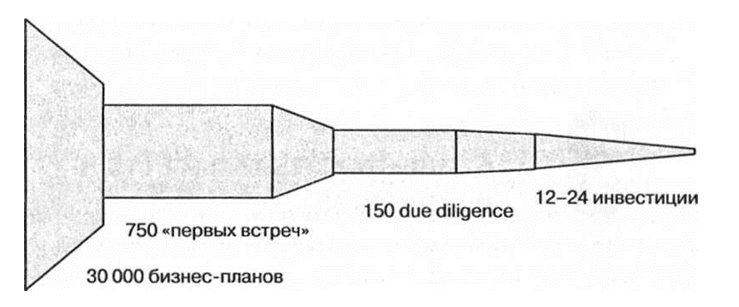
\includegraphics[scale=.6,
	%trim={<left> <lower> <right> <upper>}				
	,trim={0cm 0cm 0cm 0cm},clip	
	] {img/draper_rocket}
	\caption{Процесс отбора заявок на венчурное финансирование управляющей компанией\\ Draper Fisher Jurvetson}
\end{figure}
\end{frame}


\begin{frame}{Этапы процесса отбора компаний}
1.	Изучение поданных заявок.

2.	Первая встреча (``изучение друг друга``).

3.	Обсуждение продукции, рынка, перспектив, команды.

4.	Обсуждение вопросов интеллектуальной собственности.

5.	Обсуждение производства и выезды для осмотра производства.

6.	Обсуждение финансового состояния компании и условий инвестирования.

7.	Обсуждение, анализ и корректировка бизнес-плана.

8.	Финальная встреча.
\end{frame}

\subsection{Документы о бизнес предложении}
\begin{frame}{Документы о бизнес предложении}
\begin{itemize}
	\item[1)] резюме; 
	\item[2)] бизнес-план; 
	\item[3)] презентация.
\end{itemize}
\end{frame}

\begin{frame}{Структура бизнес плана}
\begin{itemize}
	\item[1)] ключевая информация о проекте;
	\item[2)] команда;
	\item[3)] бизнес и стратегия;
	\item[4)] интеллектуальная собственность;
	\item[5)] производство;
	\item[6)] финансы;
	\item[7)] инвестиции.
\end{itemize}
\end{frame}

\begin{frame}{Частые ошибки претендентов на инвестиции}
\begin{itemize}
	\item[1)] описание изделий/технологий дается с применением узкотехнических и специальных терминов;
	\item[2)] 	слабо проработана маркетинговая концепция и стратегия сбыта;
	\item[3)] 	недостаточное внимание уделяется вопросам управления и персонала;
	\item[4)] 	недостаточное внимание уделяется вопросам интеллектуальной собственности;
	\item[5)] 	информационная перегруженность.
\end{itemize}
\end{frame}

\begin{frame}{Частые ошибки при подготовке презентаций}
\begin{itemize}
	\item[1)] большое количество мелкого текста;
	\item[2)] неправильная цветовая гамма;
	\item[3)] большое внимание к узкоспециальным вопросам;
	\item[4)] отсутствие рисунков и фотографий или, наоборот, перегруженность дополнительными рисунками и фотографиями.
\end{itemize}
\end{frame}

\begin{frame}{Бизнес и стратегия}
\begin{itemize}
	\item[1)] сущность бизнеса компании;
	\item[2)] рынок продукции и услуг компании;
	\item[3)] конкуренты и конкурентные преимущества;
	\item[4)] маркетинг и система продаж;
	\item[5)] отраслевые риски.
\end{itemize}
\end{frame}


\begin{frame}{Цели венчурного проекта}
\begin{itemize}
	\item[1)] лидерство в определенном сегменте рынка;
	\item[2)] создание сильного бренда;
	\item[3)] рост капитализации компании в год (в зависимости от стадии): seed – 100\%, start-up – 80\%, early stage – 60\%, expansion – 40\%.
\end{itemize}
\end{frame}


\begin{frame}{Инвесторы отдают преимущество следующим проектам}
\begin{itemize}
	\item[1)] рост – не менее 15\% в год;
	\item[2)] наличие большого количества потребителей;
	\item[3)] высокий ``барьер для входа`` конкурентов.
\end{itemize}
\end{frame}

\begin{frame}{Частые ошибки предпринимателей}
\begin{itemize}
	\item[1)] нет сравнения с современными аналогами;
	\item[2)] не доказаны технические и технологические долгосрочные преимущества проекта;
	\item[3)] замалчивается решение трудных вопросов;
	\item[4)] просчитан только оптимистичный сценарий.
\end{itemize}
\end{frame}

\subsection{Особенности отбора компаний}
\begin{frame}{Особенности отбора компаний}
\textbf{- венчурными фондами:} расходы фонда на due diligence до 100 тыс. долл., формализованный процесс, включающий финансовый, операционный, налоговый, юридический анализ и анализ рынка.

\textbf{- в бизнес-ангельском секторе:} неформальный подход, основное внимание уделяется именно главной идее и общему ``видению`` предпринимателем своих будущих перспектив, поиск бизнес-ангела через сеть составляет 140 долл. за рассмотрение проекта и 2-5\% от суммы инвестиций.
\end{frame}

\begin{frame}{Особенности отбора компаний}{Российская практика}
- грамотно составленный бизнес-план – это серьезное конкурентное преимущество в глазах инвестора;

- слабое место большинства российских бизнес-планов – описание рынка, обоснование его роста, результаты маркетинговых исследований;

- государственный орган может имеет право на безвозмездную лицензию на патент и передачу ее конкурентам;

- связи с иностранным рынком, иностранные инвесторы, зарубежные патенты, рекомендации от партнеров из развитых стран - важные конкурентные преимущества.
\end{frame}

\begin{frame}{Предпочтительные проекты для российских инвесторов}
\begin{itemize}
\item	прогнозируемая доходность проекта – 50\% и выше;
\item	текущий рост рынка – 15\% в год;
\item	ожидаемый рост капитализации компании – более чем в 5 раз в течение 5 лет.
\end{itemize}
\end{frame}


\end{document}